\documentclass[a4paper, 11pt]{article}
\usepackage[utf8]{inputenc}
\usepackage[left=2cm,right=2cm,top=2cm,bottom=2cm]{geometry}
\usepackage{graphicx}

% Maths
\usepackage{amsmath}
\usepackage{amssymb}

% Double quotes
\usepackage[english]{babel}
\usepackage[autostyle, english = american]{csquotes}
\MakeOuterQuote{"}

% Tables
\usepackage{multirow}
\usepackage{longtable}
\usepackage{booktabs}

% Code
\usepackage{listings}

\usepackage{xcolor}
\usepackage{float}

\definecolor{codegreen}{rgb}{0,0.6,0}
\definecolor{codegray}{rgb}{0.5,0.5,0.5}
\definecolor{codepurple}{rgb}{0.58,0,0.82}
\definecolor{backcolour}{rgb}{0.95,0.95,0.92}

\lstdefinestyle{mystyle}{
    backgroundcolor=\color{backcolour},   
    commentstyle=\color{codegreen},
    keywordstyle=\color{magenta},
    numberstyle=\tiny\color{codegray},
    stringstyle=\color{codepurple},
    basicstyle=\ttfamily\footnotesize,
    breakatwhitespace=false,         
    breaklines=true,                 
    captionpos=b,                    
    keepspaces=true,                 
    numbersep=5pt,                  
    showspaces=false,                
    showstringspaces=false,
    showtabs=false,                  
    tabsize=2
}

\lstset{style=mystyle}

\title{Nature-Inspired Computation Report}

\author{Jordan Peters}
\date{December 2021}

\begin{document}

\maketitle

\begin{abstract}

    We analyse the effect of different parameters with the ant colony optimisation algorithm on a bin packing problem.

\end{abstract}

\begin{center}
    680041507

    I certify that all material in this report which is not my own work has been identified.

    
\includegraphics[width=100px]{figs/sig.png}
\end{center}

\section{Question 1}

\begin{figure}[h]
    \centering
    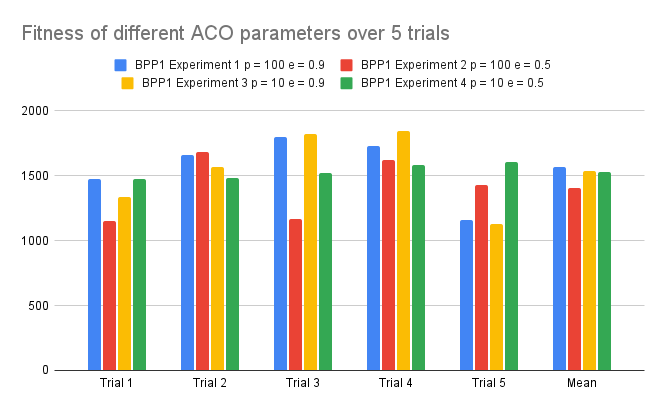
\includegraphics[width=0.7\textwidth]{figs/fitness bar charts.png}
    \caption{The resulting fitness values for each experiment and trial for BPP1. (Lower is better.)}
    \label{bpp1-bar-chart}
\end{figure}

In Figure \ref{bpp1-bar-chart} we can see that the parameters of Experiment 2 (p = 100 and e = 0.5) seem to provide the best results on average. However, Experiment 3 (p = 10 and e = 0.9) in one of its trials reached the lowest fitness value out of all models. A better description of the data can be found in the boxplots in Figure \ref{boxplots}.

\begin{figure}[h]
    \centering
    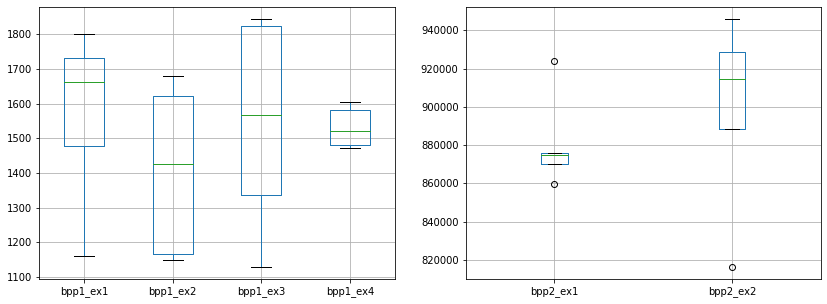
\includegraphics[width=0.7\textwidth]{figs/experiment boxplots.png}
    \caption{The distribution of fitness values over 5 trials for each experiment. EX1, p = 100, e = 0.9. EX2, p = 100, e = 0.5. EX3, p = 10, e = 0.9. EX4, p = 10, e = 0.5. BPP1 uses 10 bins and item values as $i$ between 1 and 500. BPP2 uses 50 bins and item values are $i^2$. (Lower is better.)}
    \label{boxplots}
\end{figure}

Figure \ref{boxplots} elucidates the strengths of the models. It confirms that Experiment 2 is, generally, the best model. It provides the best results the majority of the time. However, it is less optimal than Experiment 3. Experiment 4 is highly consistent, and is the most consistent of all the models.

In BPP2, Experiment 1 continues to be more consistent than Experiment 2, and Experiment 2 finds the best solution out of the two of them.

\begin{figure}[h]
    \centering
    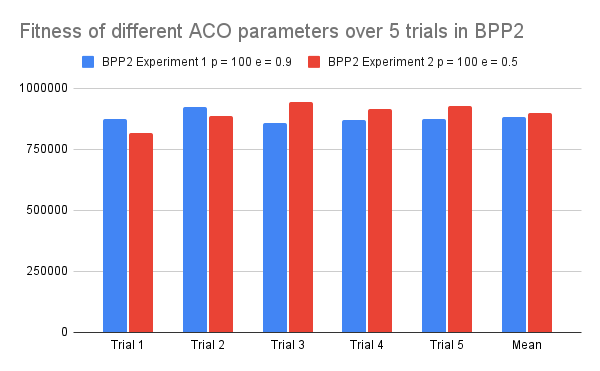
\includegraphics[width=0.7\textwidth]{figs/bpp2 fitness bar charts.png}
    \caption{The resulting fitness values for each experiment and trial for BPP2. (Lower is better.)}
    \label{bpp2-bar-chart}
\end{figure}

\section{Question 2}

The $e$ (evaporation rate) and $p$ (paths travelled before pheromone update) parameters control how aggressively the algorithm exploits the more optimal local solutions it finds. This usually leads to less globally optimal solution however, as shown in Experiments 1 and 4. In fact, 'middleground' parameters as shown in Experiment 2 actually produce the best results as opposed to choosing the most extreme values such as in Experiment 3. This suggests that the optimal model is somewhere inbetween Experiment 2 and Experiment 3. The overly aggressive Experiment 4 and the overly passive Experiment 1 show this.

I would hypothesize that this is because less solutions that could lead to globally optimal ones are evaluated as $p$ decreases, and if $e$ is a low value, this effect is even worse as locally better solutions are more biased to be evaluated because they are stronger. This is shown in Experiment 2 and Experiment 4's distributions.

For BPP2, due to the weights being squared, the performance of the models differs more drastically, but the relationships seem to transfer over.

\section{Question 3}

In terms of specific relationships for what parameter causes what, it seems higher $e$ values lead to more globally optimal solutions but are less consistent, as local solutions are less biased. Lower $p$ values do not have a similar 'linear' relationship. It seems that the way $p$ affects fitness changes based on the value of $e$. In practice, $p$ increases the amount that stronger paths are evaluated.

In Experiments 2 and 4 we see $p$ decreasing cause less globally optimal but more consistent results, converging into a local optimum. The lower $p$ value gives worse performance.

In Experiments 1 and 3 however, we see Experiment 3 reach better global optimums, and seemingly more often. However it's more inconsistent than Experiment 1. The lower $p$ value gives better performance.

The higher the $p$ value, the more aggressively locally optimal solutions are travelled. The lower the $e$ value, the more aggressively locally optimal solutions are travelled. It is better for both to be aggressive than there to be a mismatch, but should there be a mismatch, global solutions are better found with more paths and high evaporation rate than less paths and low evaporation rate.

\section{Question 4}

Neural networks use hidden layers and reinforcement learning via a fitness function to learn how best to perform an algorithm \cite{gurney2018introduction}. Instead of modelling a graph, the neural network would directly learn from randomly placing items in bins, and create its own relationship with the problem within its hidden layer of neurons. This could provide competitive results against ant colony optimisation because the neural network could form its own local heuristic that's different from the 'pheromone system' in ACO that could perform better for this problem. It would only be clearly worse in that the explainability of neural networks is challenging.

\section{Conclusions and Further Experiments}

In conclusion, $p$ and $e$ affect the algorithm's ability to reach more globally optimal solutions. The best parameters appear to lie somewhere close to p = 100 and e = 0.5. Lower $p$ and higher $e$ values collectively allow for better solutions to be more likely to be found and exploited, but cause the model to be much more inconsistent.

For further experiments, we decided to plot $p$ and $e$ and the resultant fitness values onto a 3D graph, as well as try new $p$ and $e$ values based on the observations we saw in the initial 3D graph. Through this, we attempt to analyse the solution space. The graph is shown in Figure \ref{furtherexperiment2}. First, we analysed the visual midpoint of the four initial solutions (e = 0.7, p = 60), and then we plotted beyond the initial data's range (e = 0.25, p = 125). The rationale is that exploring the midpoint, then exploring further points, will show us a decent impression of the solution landscape.

\begin{figure}[h]
    \centering
    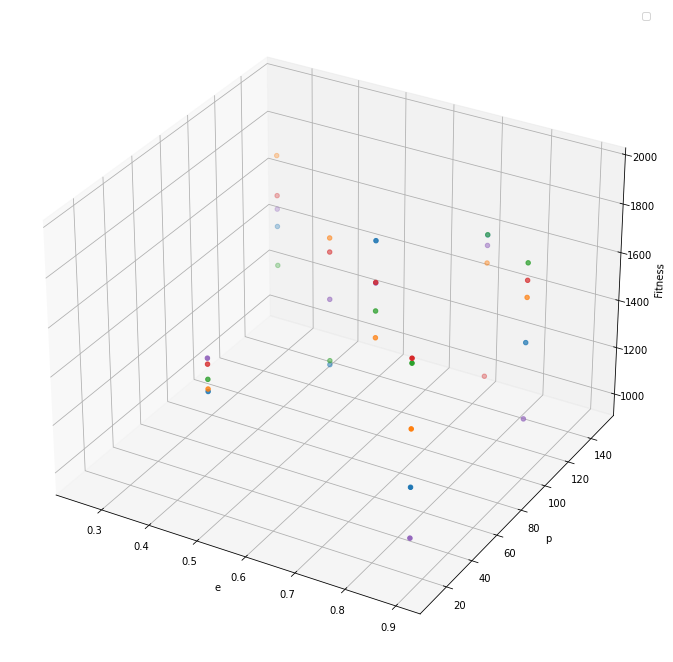
\includegraphics[width=0.7\textwidth]{figs/furtherexperiment2.png}
    \caption{The resulting fitness values for each experiment and trial for the further experiments. (Lower is better.)}
    \label{furtherexperiment2}
\end{figure}

As a result of this further experiment, our new global optimal at e = 0.7, p = 150 was found! An evolutionary algorithm could be applied to this problem to further search the solution landscape, but already we are seeing increasingly better and more consistent successes as we adjust the parameters.

\bibliographystyle{IEEEtran}
\bibliography{report}


\end{document}
